\section{Results}
In the following paragraphs the results of the simulation study are presented and discussed with constant reference to the possible clinical application of the CLaRyS Compton camera system as particle therapy monitor. The clinical implementation of such a monitoring system has been tested with the simulation of clinical proton and carbon ion beams, with realistic spatial and time structure reproducing two accelerators at present employed for treatments~\ref{subsubsection:modelisation_fasceau_ions_CC_hadrontherapy_Geant4}. As preliminary study, the detection efficiency of the camera has been tested with the simulation of the irradiation with point-like gamma sources in different position with respect to the center of the camera. After that, the beam exposure has been simulated with different beam intensities for an analysis of the clinical-like detection environment (background, random coincidence contamination), in order to focus in the end on the event reconstruction with the comparison of two different methods (line-cone analytical reconstruction and MLEM iterative algorithm) and on the estimate of the camera precision in the identification of the fall-off of the dose profile.


\subsection{Compton camera absolute efficiency}
\label{Results::efficiency}

The absolute efficiency is crucial for the Compton camera performances and for its possible application in treatment monitoring. As already mentioned in section~\ref{section::Intro}, an efficient monitoring system should be ideally in real time, in order to allow for a treatment adaptation or interruption in case of severe issues detected in the delivered dose profile with respect to the planned treatment. In order to achieve an online detection of such deviations, given the reduced prompt gamma emission rate per incident ion~\cite{Ortega:2015aa}, an high detection efficiency is required to perform a monitoring on, ideally, a beam spot basis. In addition to this, the absolute detection efficiency directly affects the image reconstruction quality, which is in general increased for increased statistics.\\
In order to well define the expected camera efficiency, it has been studied with the irradiation from point-like monoenergetic gamma sources, set in different positions with respect to the center of the camera on the transverse plane.	\\
The absolute efficiency $\epsilon$ is defined as:
\begin{equation}
\epsilon =\frac{N\gamma_{recons}}{N\gamma_{total}},
\end{equation}
\label{eq:equation_efficacite_absolue}
with $N\gamma_{recons}$ the number of gamma events in coincidences,\newline
\hspace*{1cm}$N\gamma_{total}$ the total number of gamma emitted: $10^8$.\newline

The setup is the same as figure \ref{fig:fig_setup_CC_simulation_Hadronth}, with the exception of the PMMA phantom which is removed to leave the gamma source in air.
The point source is set in the range $-300$~mm to $+300$~mm (with the center of the camera transverse section set in the position 0) with a step of 20~mm close to the center of the camera, then increasing up to 1~cm for the most peripheral point. The movement followed the transverse axis of the camera. Different energies has been tested to mimic different prompt gamma spectroscopic lines: 300~keV, 500~keV, 1~MeV, 2~MeV, 4~MeV, 6~MeV.\newline
The obtained results are shown in figure \ref{fig::efficiency_study}. On the left side, we show the results achieved with an ideal detector, while on the right side realistic energy cuts are applied on each detector section: the lower energy limit  has been set to 50~keV for the scatterer and 100~keV for the absorber.

\begin{figure} [!hbtp]	
\centering
\subfloat[]{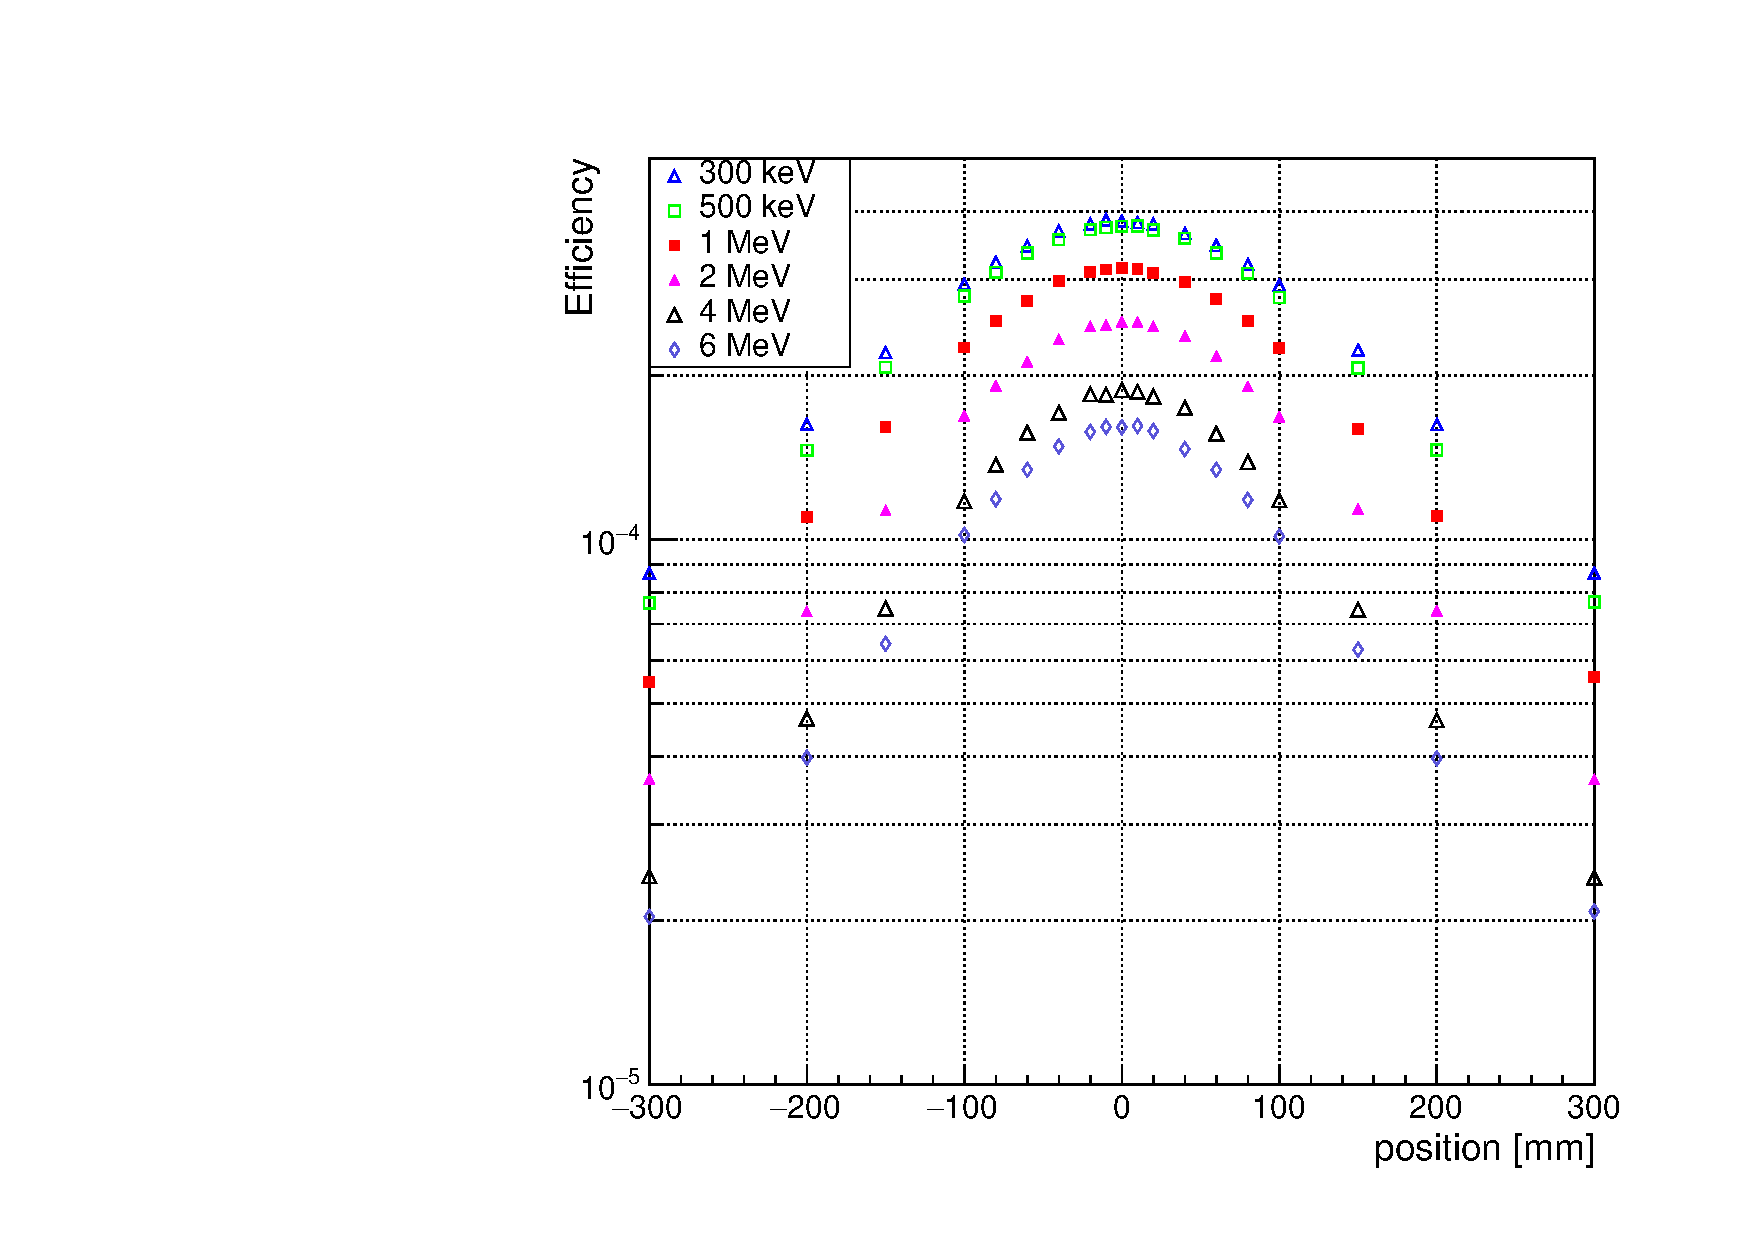
\includegraphics[width=0.5\textwidth]{./Figure/EffVSpos.pdf}}
\subfloat[]{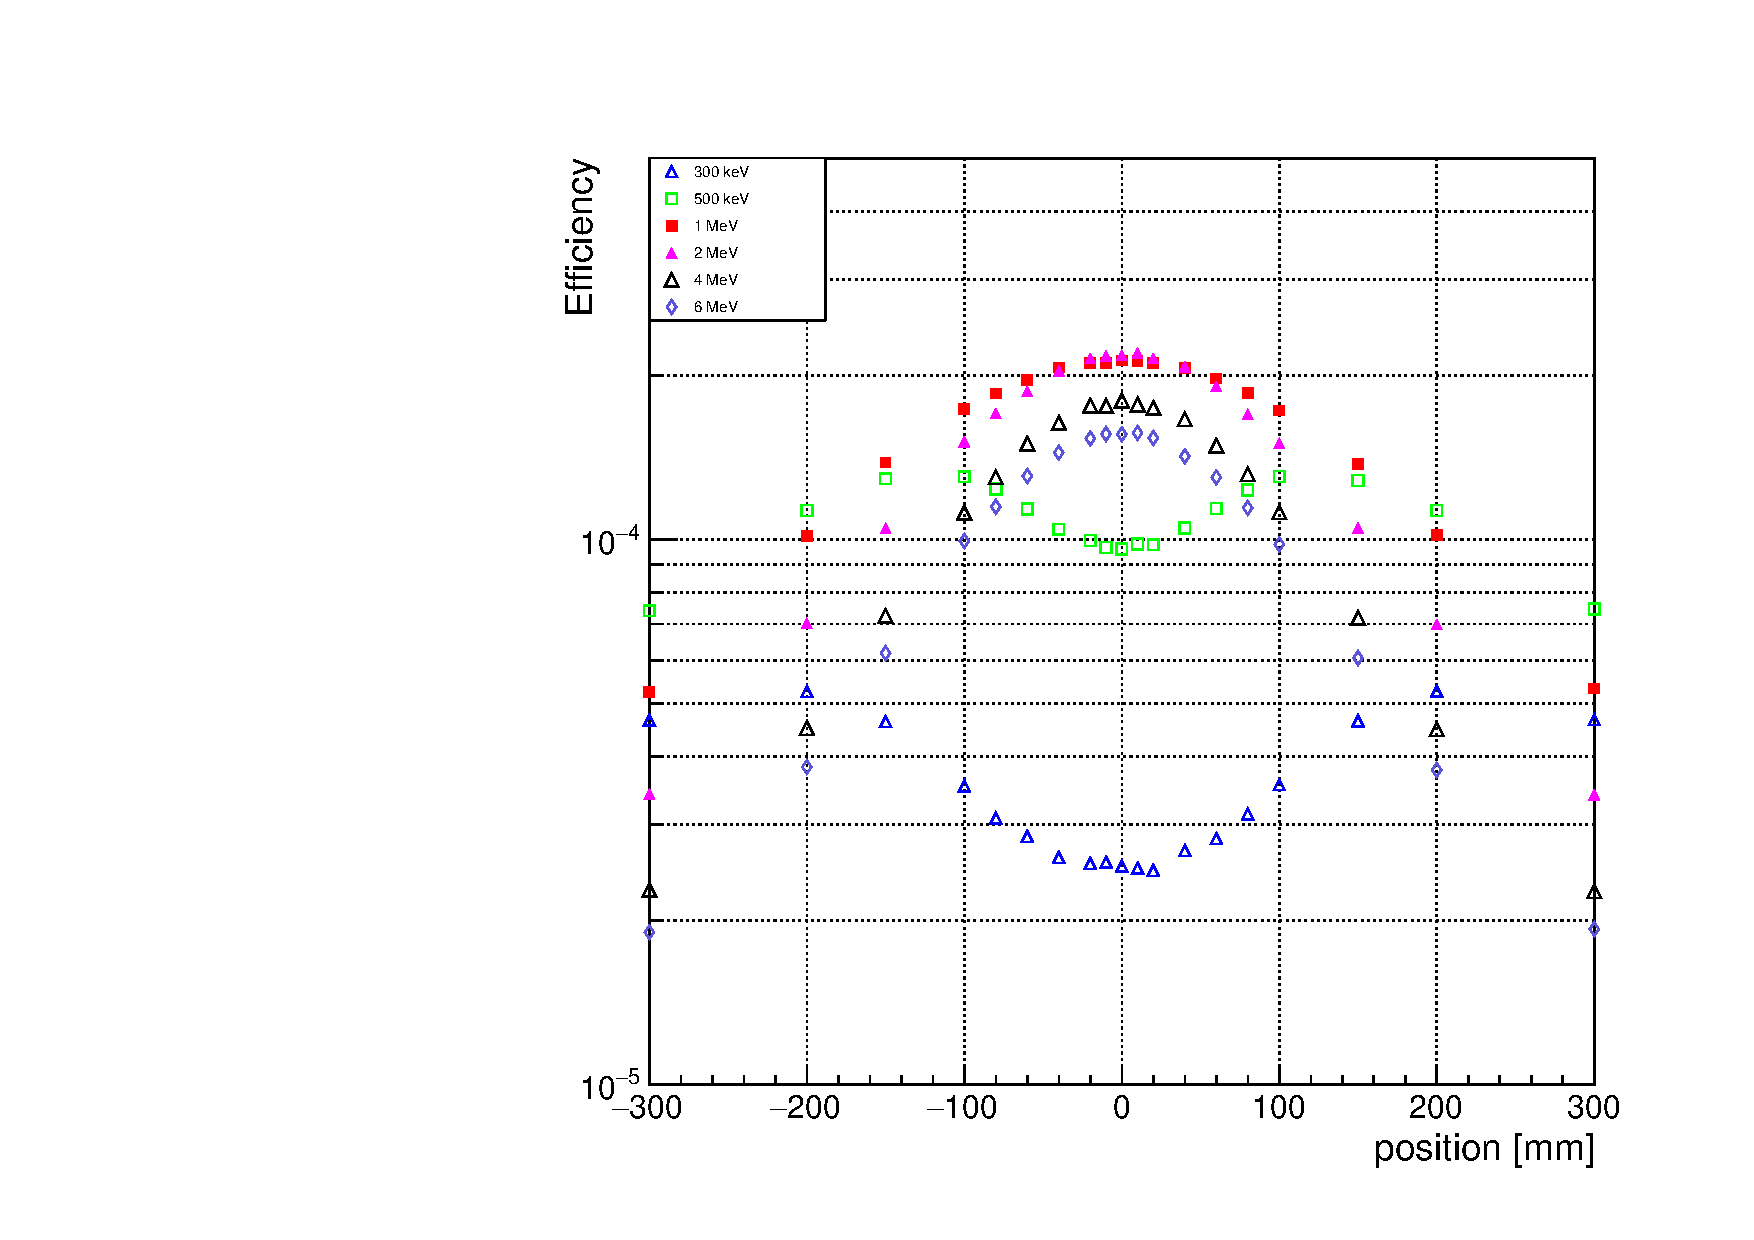
\includegraphics[width=0.5\textwidth]{./Figure/EffVSpos_withCut.pdf}}
\caption{Absolute Compton camera efficiency as a function of the gamma source position for different gamma energies, in the range between 300~keV to 6~MeV. The left side shows the camera efficiency without any applied energy cut. It models an ideal Compton camera. In the right side, detector energy cuts are applied: the lower energy thresholds are set to 
50~keV for the scatterer and 100~keV for the absorber, to reproduce realistic scenario. This values can change for the final detector configuration, according to the detector energy resolutions achieved.}
\label{fig::efficiency_study}
\end{figure}

As expected according to the interaction probability energy dependency, the efficiency is higher for low gamma energies, and it lies in the range $4\times10^{-4}$ at 300~keV and $1.5\times10^{-4}$ at 6~MeV (figure \ref{fig::efficiency_study}). Moreover, it can be noticed how the efficiency quickly drops quickly as the point source drifts away from the camera center: this effect is more important for high energies, for which the incident gamma is less deflected in the scatterer for the same energy deposited compared to a low energy gamma (see equation~\ref{Compton_equation}). Therefore, considering 1~MeV as the average and reference gamma energy for ion beam therapy monitoring, the Compton camera position optimization with respect to the expected Bragg peak position appears mandatory for an efficient fall-off reconstruction.\newline
Regarding the applied energy cuts, figure~\ref{fig::efficiency_study}(b) clearly shows an important effect on low energy gammas in the central area of the camera. The effect is negligible for positions with a distance greater than 200~mm from the center of the camera, and for any distance at energies above 2~MeV. A further study showed how this effect is mainly due to the cut applied on the scatterer detector. Indeed, for low energies, below 2~MeV, the increased efficiency in the central section of the camera active surface shown in figure~\ref{fig::efficiency_study}(a) is linked to the increased relative number of photons approaching the camera with small angles. These photons are more likely undergoing Compton scattering with a reduced energy deposition, which is recorded by an ideal detector and rejected by the energy cut. The effect is all the more important as the primary gamma energy is limited, creating the peculiar energy dependence of the efficiency reduction emerged in the results in figure~\ref{fig::efficiency_study}(b).\\ 

\subsection{Beam intensity}
\label{Results::beamInt}

As the Compton detection principle relies on time coincidences, in addition to the main importance played by the detectors energy resolutions, the beam intensity and time structure are important parameters to be studied in order to asses the possible clinical implementation of a Compton detection based monitoring of ion beam treatment. In the simulation, the beam intensity is modeled by an average number of particles per bunch. The exact number of particles in each bunch is given by a random extraction from a Poisson distribution, where the mean value is the selected beam intensity. The range of intensities is defined in order to cover a wide range of operation: from a very low beam intensity to a realistic, clinical particle rate. Therefore, for proton and carbon ions, the lowest beam intensity is set to 0.1 particles per bunch on average, while the upper limit is set to 217 protons or 70 carbon ions per bunch. For the analysis of the results, the coincidence yields are scaled to the number of incident ions and the beam intensity to the average number of ions per bunch.\\ 
In figure~\ref{fig:coincidences} the different components of the resulting secondary signal are shown as a function of the beam intensity. The true coincidences represent detector time coincidences generated by the same gamma ray. All the other coincidence types compose the background. All the simulations are performed with $10^{8}$ primary protons and  $2\times10^{5}$ primary carbon ions. Those value correspond to realistic clinical values used for the treatment of a single spot. The collected data sets are reported with and without the applied time-of-flight discrimination, mainly employed for neutron rejection, as mentioned in section~\ref{MatMeth::TOF_Ecut}.\\

\begin{figure} [!h]
\caption{Coincidences yield for protons (left) and carbon ions (right) as a function of the beam intensity. The intensity is reported as number of incident particles per bunch. The filled markers correspond to the collected data without time-of-flight discrimination, while this cut is applied to the data reported with empty markers. Moreover, the yields are given before and after the profile reconstruction with the line cone algorithm.}
\subfloat[]{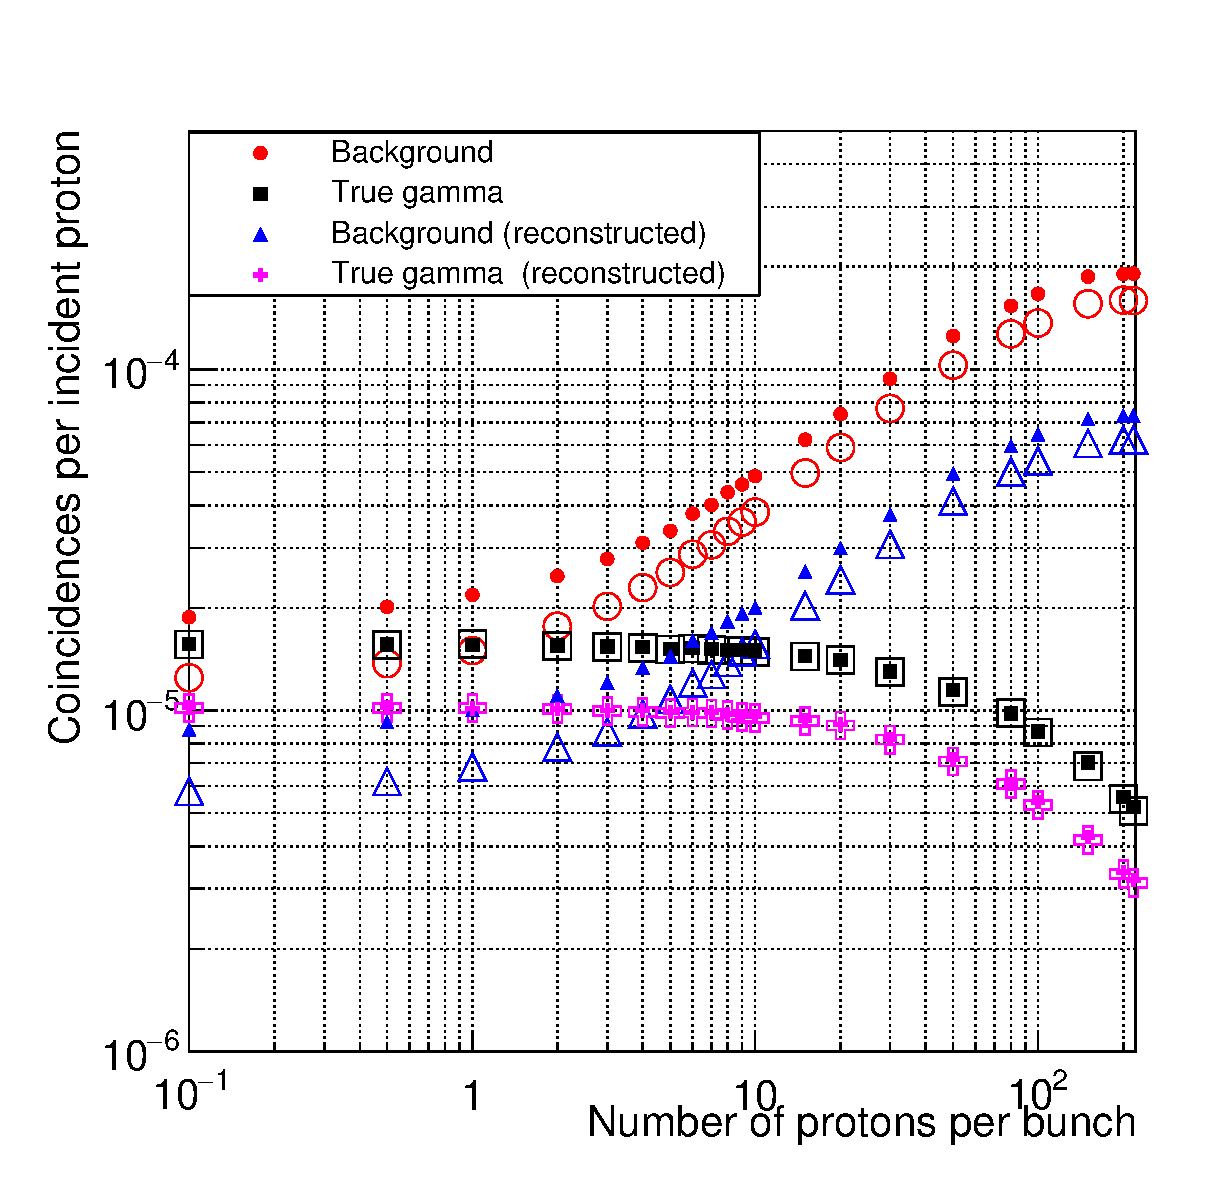
\includegraphics[width=0.5\textwidth]{./Figure/2017_06_28_Taux_coincidences_variation_protons_New_design_4EntreesLegend_LogXLogY.eps}}
\subfloat[]{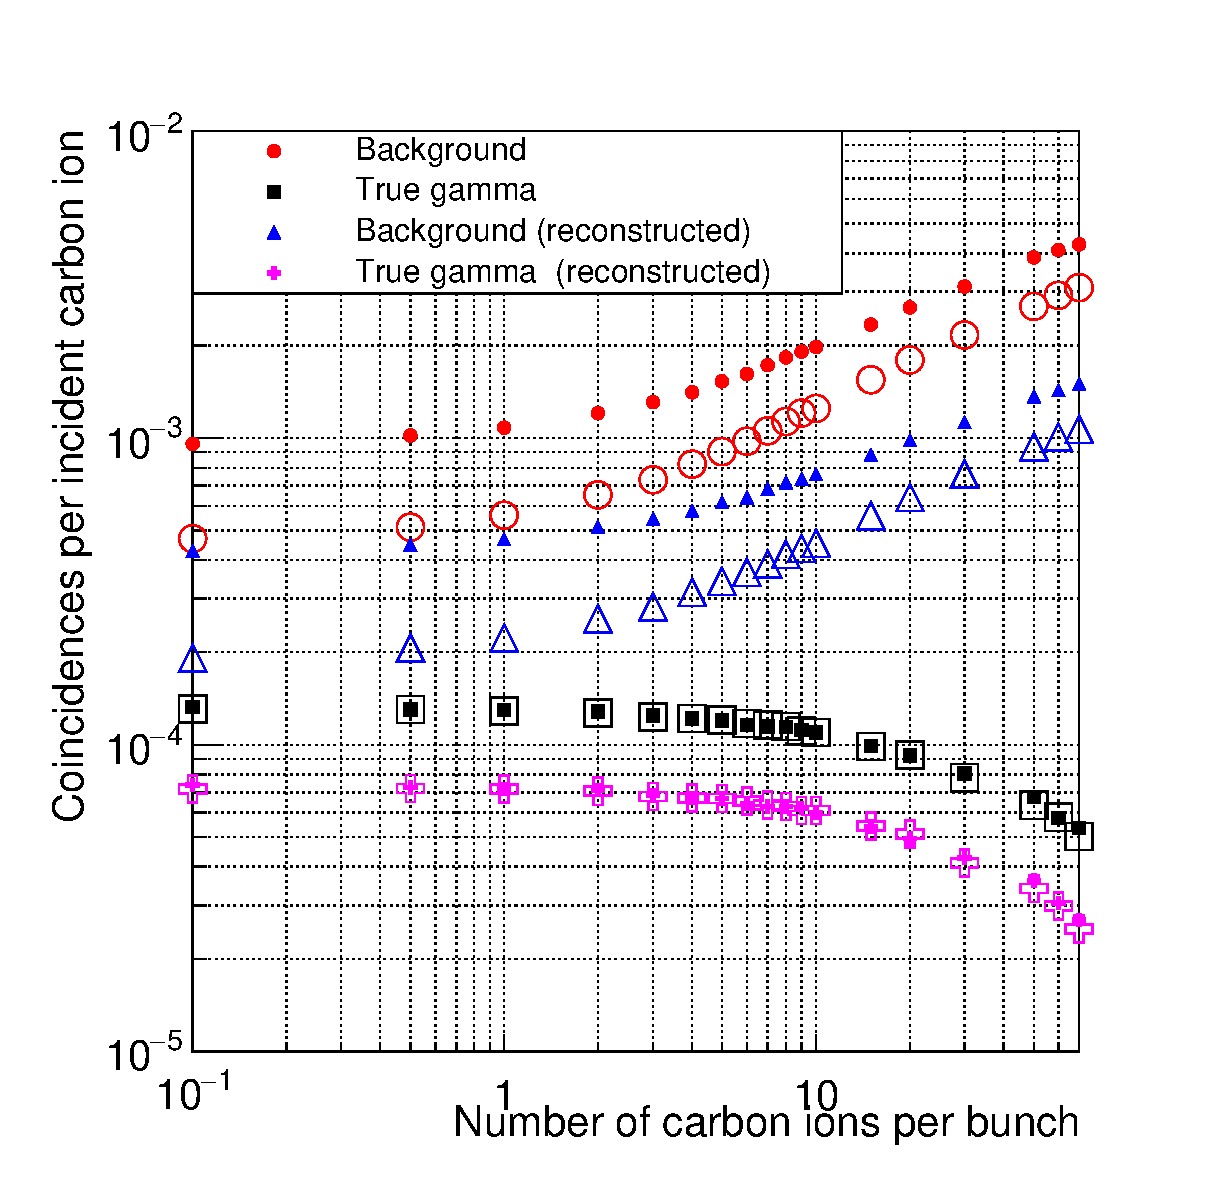
\includegraphics[width=0.5\textwidth]{./Figure/2017_06_28_Taux_coincidences_variation_carbonIons_New_design_4EntreesLegend_LogXLogY.eps}}
\label{fig:coincidences}
\end{figure}

At the clinical beam intensity, the high background level is mainly due to the random coincidences. In fact, the probability to detect two radiation coming from two different incident particles increases with the number of incident particles per bunch. Another issue is the single rate of events detected by each detector at those high intensities. For instance, at the clinic beam intensity in proton therapy, the single rate on the absorber is around 300 MHz and on the first silicon layer it is around 20 MHz. The current electronic front end and acquisition system are not able to treat this amount of data coming from all the detectors. As a result, it appears that it is impossible to use the Compton camera at a clinical beam intensity for the treatment monitoring in ion therapy.\newline
Nevertheless, if the intensity decreases enough to avoid almost all the random coincidences, the monitoring seems more feasible. In addition, it can be supposed that the time of flight discrimination will improve the signal to the background ratio at low intensities by suppressing the coincidences induced by charged particles. Indeed, the charged particles are slower than gamma rays which move at the light speed.

\subsection{Comparaison LM-MLEM vs Line cone reconstruction}
\label{Results::reconstruction}

\begin{figure} [!h]
\subfloat[]{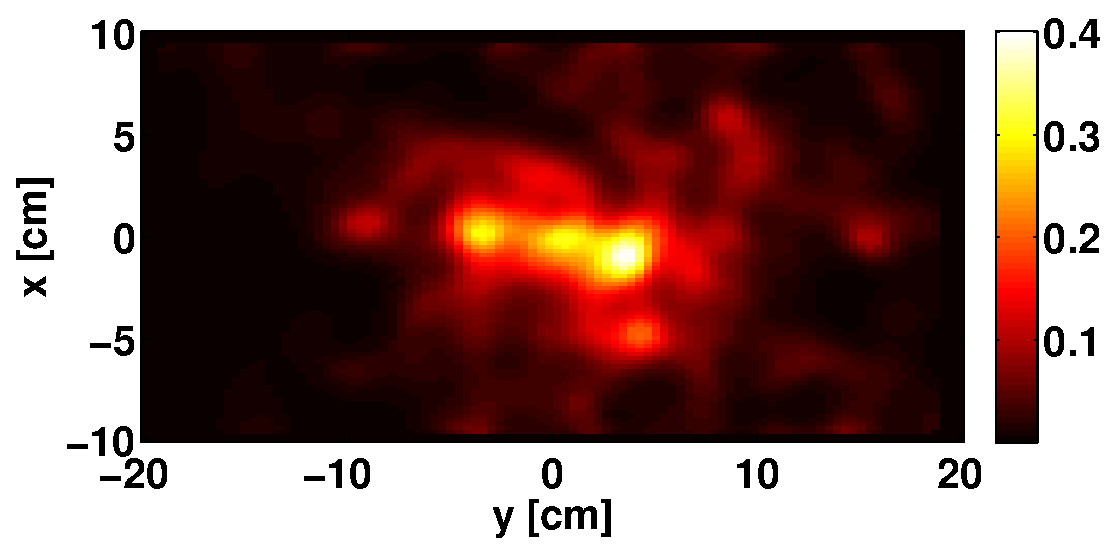
\includegraphics[width=0.5\textwidth]{./Figure/MLEM_2D.pdf}}
 \subfloat[]{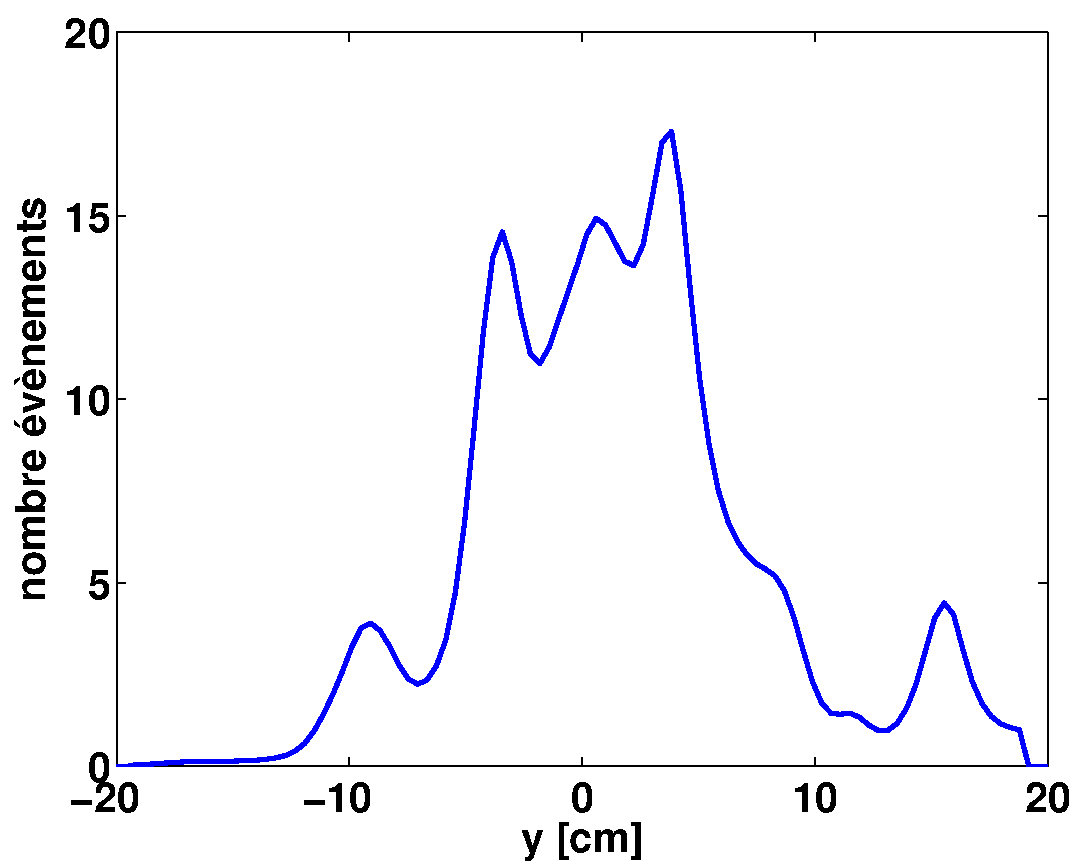
\includegraphics[width=0.5\textwidth]{./Figure/MLEM_1D.pdf}}\\
  \subfloat[]{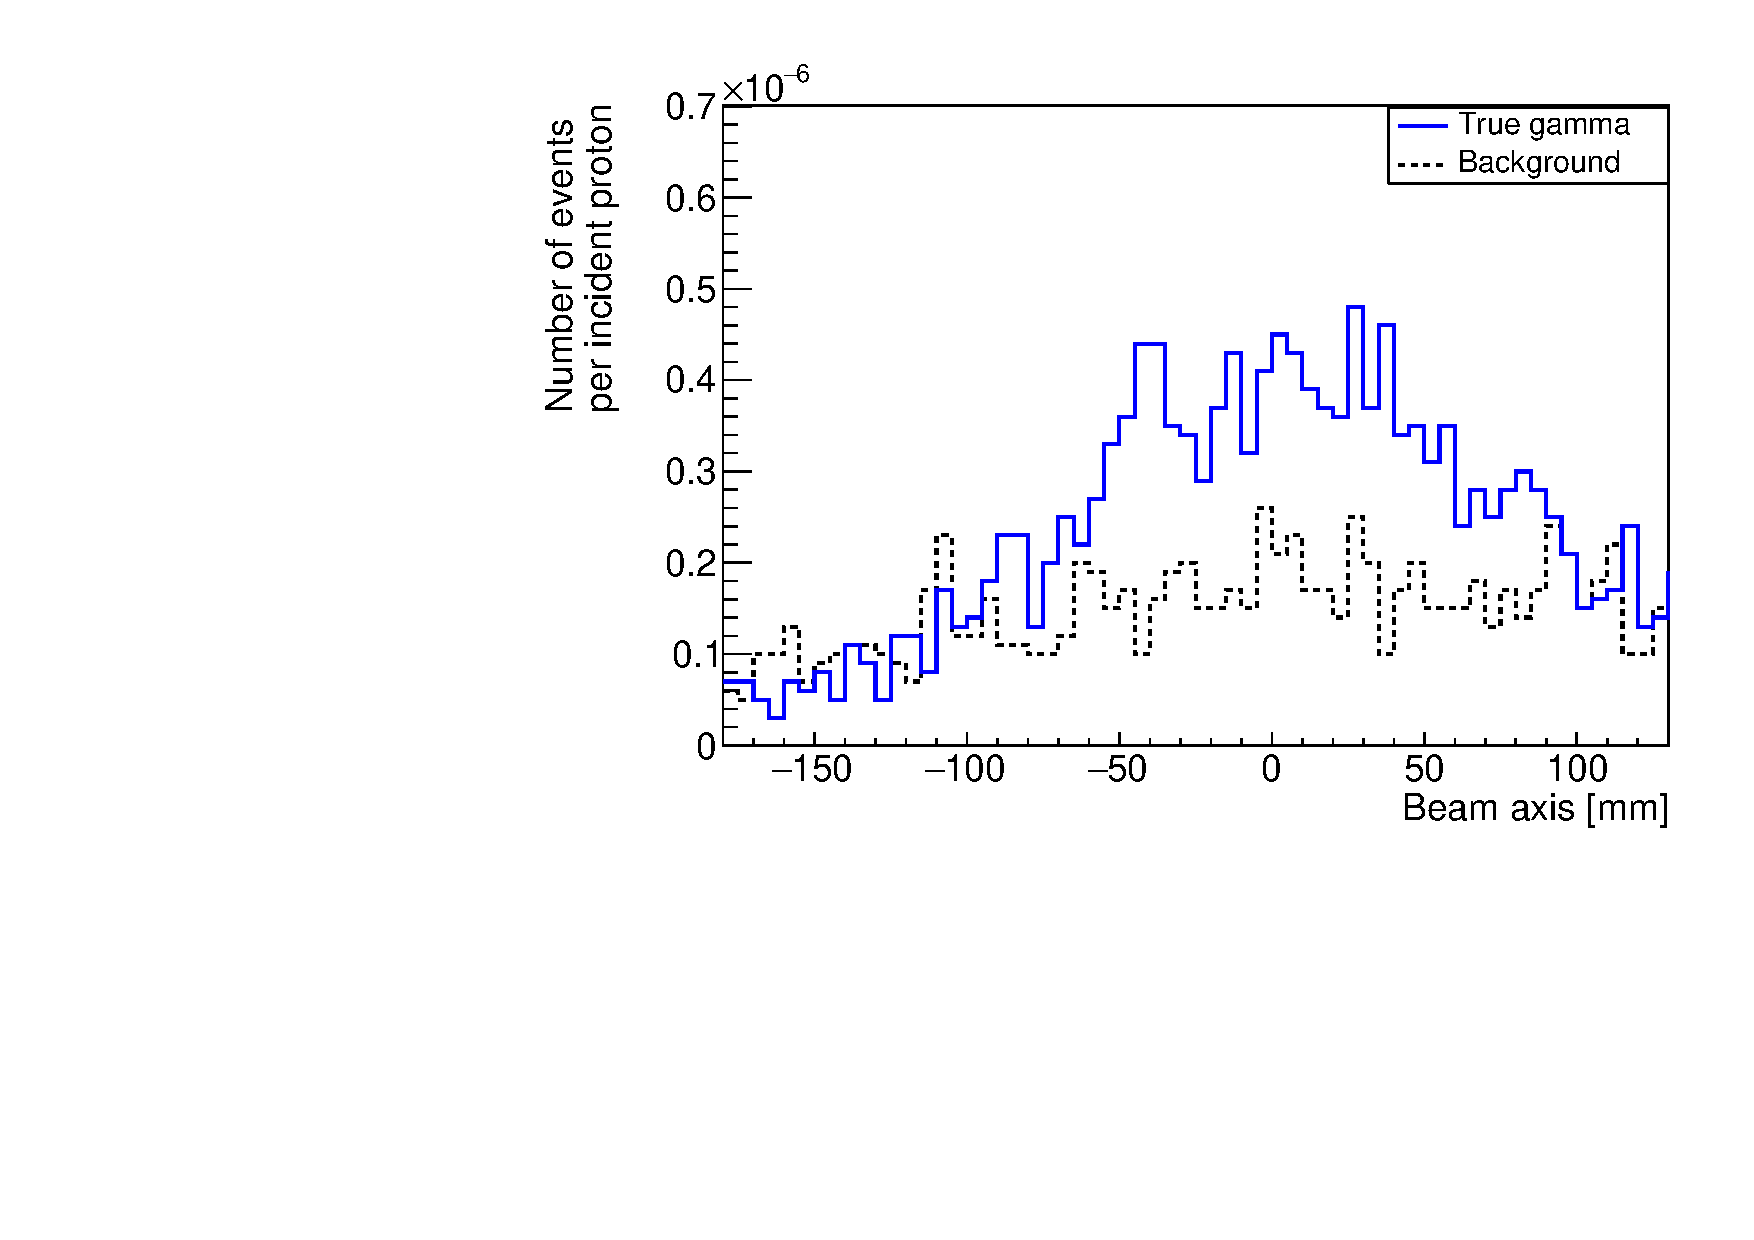
\includegraphics[width=0.5\textwidth]{./Figure/2015_02_16_Reconstruction_coinc_160MeVProton_TOF_6ns_file0to100_zoom.pdf}}
  \label{fig:comparaison}
\caption{LM-MLEM reconstruction for a proton beam at 160 MeV and $10^{8}$ incident protons. The events are detected in coincidence and the beam intensity is reduced to 1 proton per bunch. The PMMA target has a diameter of 15 cm and is 20 cm long. The Compton camera is centred at $y=+50 mm$. The time of flight discrimination is applied and 20 iterations are realized. The figure \ref{fig:fig_MLEM_CC_simulation_Hadronth_proton_reconstruction} represents the reconstruction in 2D for the plan (x,y). The position $x=0 mm$ is the center of the PMMA phantom and y axis the direction of the proton beam. The figure \ref{fig:fig_MLEM_CC_simulation_Hadronth_proton_profil} shows the profil corresponding to the figure \ref{fig:fig_MLEM_CC_simulation_Hadronth_proton_reconstruction} and following the axis y. The Bragg peak is localized at $y=+50 mm$. The figure \ref{fig:fig_LC_CC_simulation_Hadronth_proton_profil} is the profil obtained by means of line cone algorithm for the same simulation datas.}

\end{figure}

%   \begin{verbatim}
% a) 2015_10_20_Volume_100x100x5_voxels_and_size_20x40x1_source_Proton160MeV_camera_50mm_stat_2175events_sans_MatriceSensibility_bordYplusmoins-3_bordXplusmoins-3_median_iteration_10.
% b) 2015_10_20_Volume_100x100x5_voxels_and_size_20x40x1_source_Proton160MeV_camera_50mm_stat_2175events_sans_MatriceSensibility_bordYplusmoins-3_bordXplusmoins-3_selectionX_20mm_Filtre_median_iteration_Profil_Y_iteration_10. 
% c)  2015_02_16_Reconstruction_coinc_160MeVProton_TOF_6ns_file0to100_zoom               
%  \end{verbatim}

\subsection{Compton camera precision}
\label{Results::precision}

The information given by a control device as the Compton camera has to be viable and as precise as possible. In order to estimate the precision of the Compton camera, a method is used. 

\begin{figure}[!hbtp]	
\centering
\caption{The Compton camera precision is estimated with two different algorithms: line cone and LM-MLEM. The precision is given for $1\times10^{8}$ to $5\times10^{9}$ incident protons. A linear fit is realized in order to obtain the slope of the results (p1 parameter). The graphic is scaled in log-log. }	
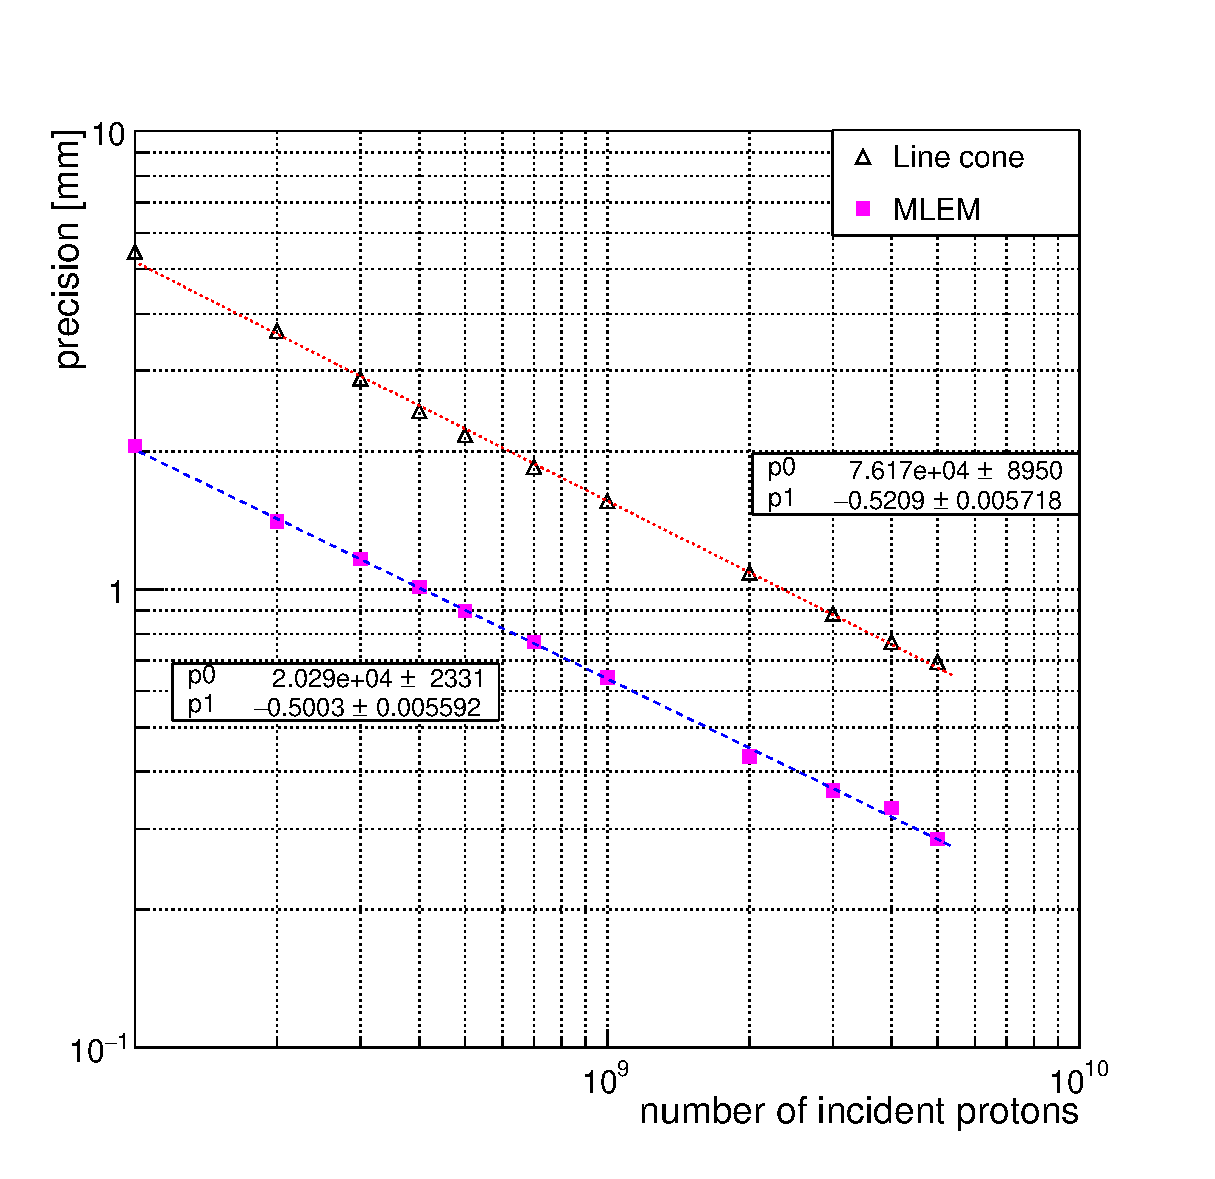
\includegraphics[width=0.7\textwidth]{./Figure/2017-10-21_Precision_Comparaison_linecone_MLEM_Article_Fit.eps}
\end{figure}



